\RequirePackage{fix-cm}
\documentclass[twocolumn]{svjour3}
\smartqed

\usepackage[T1]{fontenc}
\usepackage{mathptmx}
\usepackage{graphicx}
\usepackage{booktabs}
\usepackage{multirow}
\usepackage{threeparttable}
\usepackage{amsmath,amssymb}
\usepackage{microtype}
\usepackage[hidelinks,hypertexnames=false]{hyperref}
\usepackage{xurl}
\usepackage[section]{placeins}
\usepackage{float}
\graphicspath{{../figures/}}

\newcommand{\method}{SRPA-YOLO}
\newcommand{\mapall}{mAP@0.50:\allowbreak0.95}
\newcommand{\srpatablesize}{\footnotesize}
\newcommand{\srpatablesetup}{\srpatablesize\setlength{\tabcolsep}{3.5pt}\renewcommand{\arraystretch}{0.96}}
\setlength{\emergencystretch}{2em}
\setcounter{topnumber}{3}
\setcounter{dbltopnumber}{3}
\renewcommand{\topfraction}{0.92}
\renewcommand{\dbltopfraction}{0.92}
\renewcommand{\textfraction}{0.06}
\renewcommand{\floatpagefraction}{0.80}
\renewcommand{\dblfloatpagefraction}{0.80}
\setlength{\textfloatsep}{9pt plus 2pt minus 2pt}
\setlength{\dbltextfloatsep}{8pt plus 2pt minus 2pt}
\journalname{Journal of Real-Time Image Processing}

\begin{document}

\title{SRPA-YOLO: Shared-Representation and Private-Rank Allocation for Real-Time Small-UAV Detection}
\titlerunning{SRPA-YOLO for Real-Time Small-UAV Detection}

\author{Xianpu Wang \and Haijie Zhi \and Qing Fei}
\authorrunning{X. Wang et al.}

\institute{X. Wang \and Q. Fei \at
School of Automation, Beijing Institute of Technology, Beijing 100081, China\\
\email{3220252903@bit.edu.cn}\\
\email{feiqing@bit.edu.cn}
\and
H. Zhi \at
College of Energy Engineering, Zhejiang University, Hangzhou 310027, China\\
\email{22427029@zju.edu.cn}
}

\date{Received: date / Accepted: date}
\maketitle

\begin{abstract}
Long-range unmanned aerial vehicles (UAVs) occupy few pixels and are readily confused with background clutter, while onboard detection is constrained by memory and frame time. This study introduces Shared-Representation and Private-Rank Allocation YOLO (SRPA-YOLO), a compact one-stage detector that allocates prediction-head capacity according to task requirements. A 64-channel structurally re-parameterized representation is shared by classification and box-distribution prediction, whereas a zero-output-initialized 16-channel classification-private representation contributes an additive classification residual. This allocation makes the box output directly independent of the classification-private representation. Before deployment, the two stems and their task projections are fused algebraically into one 80-channel $3\times3$ convolution followed by one output projection. The training-time private path is thus fully absorbed into the single-path deployment graph. On the hash-deduplicated DUT Anti-UAV test set, the validation-selected checkpoint achieves 95.850\% Precision, 92.201\% Recall, 95.185\% AP@0.50, 67.071\% AP@0.50:0.95, and 77.329\% AP@0.75 with 2.164 M deployed parameters. Relative to YOLOv8n, these metrics increase by 3.088, 8.242, 5.057, 6.895, and 9.750 percentage points, respectively, while the parameter count decreases by 0.842 M. Two same-process paired measurements yield latencies of 9.7435 and 9.8574 ms for SRPA-YOLO and 9.8859 and 9.9893 ms for the paired YOLOv8n control. Under the evaluated protocol, the results indicate that constrained classification-private capacity improves the accuracy--compactness trade-off while retaining comparable frame time.
\keywords{unmanned aerial vehicle \and small-object detection \and real-time image processing \and structural re-parameterization \and knowledge distillation \and lightweight detector}
\end{abstract}

\section{Introduction}

Small unmanned aerial vehicles (UAVs) are increasingly used in logistics, inspection, emergency response, and low-altitude sensing. The same accessibility also creates a demand for vision-based detection around protected airspace. Compared with generic object detection, long-range UAV detection is unusually unforgiving: a target may cover fewer than $16\times16$ pixels after letterboxing, motion and defocus weaken its contours, and clouds, birds, buildings, and foliage generate visually similar responses. A detector must therefore raise recall without flooding the scene with false positives, and it must do so under the memory and latency constraints of an edge platform. Recent surveys identify this accuracy--latency tension as a central problem in vision-based anti-UAV systems \cite{yasmeen2025review,wang2021smallobjectsurvey}.

One-stage detectors such as YOLO and SSD established direct dense prediction as a practical route to real-time detection \cite{redmon2016yolo,liu2016ssd}. Feature-pyramid and path-aggregation designs subsequently improved the exchange of high-level semantics and fine spatial details \cite{lin2017fpn,liu2018panet}. Anchor-free formulations and quality-aware classification further reduced hand-designed priors and aligned confidence with localization quality \cite{tian2019fcos,lin2017focal,li2020gfl}. Yet simply increasing the number of high-resolution branches or stacking attention modules can increase memory traffic and kernel-launch overhead. EfficientDet, YOLOv4, and YOLOv7 demonstrate that practical speed depends on coordinated backbone, neck, training, and deployment design rather than FLOPs alone \cite{tan2020efficientdet,bochkovskiy2020yolov4,wang2023yolov7}.

The central observation of this study is that classification and localization do not require identical feature subspaces. Classification favors semantic invariance and inter-class discrimination, whereas localization must preserve boundary- and displacement-sensitive information. TSD showed that a common proposal and representation can induce task conflict \cite{wu2020tsd}, and TOOD demonstrated the value of combining task interaction with task-specific features and alignment \cite{feng2021tood}. A fully decoupled head reduces direct feature competition but duplicates costly spatial processing. Conversely, a fully shared head is compact but constrains both tasks to the same representation budget. These considerations motivate a constrained alternative: retain a compact basis for both tasks and allocate a small additional representation only to classification.

We therefore propose \method{}, short for Shared-Representation and Private-Rank Allocation YOLO, as a structural modification of the YOLOv8 one-stage framework. YOLOv8n serves as the primary baseline for attributing changes in accuracy, parameter count, and latency. The detector retains P2--P4 feature maps through a lightweight bidirectional neck and applies a structurally re-parameterized head at each scale. A 64-channel shared stem supports box-distribution and class prediction, whereas a 16-channel classification-private stem supplies an additive class residual. Zero initialization of the private output projection preserves the shared detector's initial input--output function. Before inference, RepVGG-style structural re-parameterization \cite{ding2021repvgg} concatenates the equivalent stem kernels and merges their task projections into a single path. Classification capacity is therefore expanded during optimization without retaining a parallel private inference branch.

Training follows two stages. Stage I learns the shared detector from standard supervision and response distillation. Distribution-level localization distillation transfers the teacher's discrete box distributions \cite{zheng2022ld}, while a confidence-weighted term emphasizes reliable teacher locations. Stage II starts from the function-preserving zero-residual state and optimizes only the classification-private stem and projection. Under this constraint, the learned box function remains fixed while classification receives additional representational capacity.

The method combines constrained task-specific representation allocation, function-preserving initialization, and exact deployment fusion; task decoupling, zero initialization, distillation, and structural re-parameterization are established techniques individually. The principal contributions are as follows:
\begin{enumerate}
\item We formulate prediction-head capacity as shared and classification-private representation allocation. The resulting 64+16 design makes the box output directly independent of the private representation, while allowing classification to use the combined shared and private row spaces.
\item We introduce a function-preserving two-stage realization in which a zero-output private projection is refined after the shared detector has converged. This isolates additional classification capacity without changing the established box-regression mapping during Stage II.
\item We derive an exact fusion rule that converts the shared and private training paths into one $3\times3$ stem and one $1\times1$ output layer per scale, preserving the computed outputs up to floating-point roundoff and eliminating private-branch inference overhead.
\item A controlled evaluation with validation-selected checkpoints, IoU-resolved AP, matched Stage-II seeds 40/41/42, and same-process paired latency measurement characterizes the resulting detector. Relative to YOLOv8n, the final checkpoint improves Precision, Recall, AP@0.50, \mapall{}, and AP@0.75 by 3.088, 8.242, 5.057, 6.895, and 9.750 percentage points, respectively, while reducing deployed parameters by 28.0\%.
\end{enumerate}

\section{Related Work}

\subsection{Real-Time and Small-Object Detection}
The COCO evaluation protocol established averaged AP over intersection-over-union (IoU) thresholds as a standard measure of localization quality \cite{lin2014coco}. For small objects, however, repeated downsampling destroys both energy and phase information before a detector can form a stable response. High-resolution pyramids mitigate this loss, but their cost scales with spatial area. YOLOv8 provides a compact anchor-free implementation and reproducible training stack \cite{ultralytics2023}. Because SRPA-YOLO is developed within this framework, YOLOv8n is the primary structural and deployment baseline. YOLO11 is included as a contemporary compact control, whereas UAV-specific reproductions test whether the proposed design remains competitive beyond its parent architecture.

Hardware-aware modules reduce the cost of retaining high-resolution features. MobileNet replaces dense spatial convolution with depthwise separable operations \cite{howard2017mobilenets}; GhostNet synthesizes redundant features through cheap transforms \cite{han2020ghostnet}; FasterNet argues that realized FLOPS and memory access are as important as nominal FLOPs \cite{chen2023fasternet}. Our backbone and neck use C2f aggregation, Ghost convolution, depthwise downsampling, and a partial-convolution stage in this spirit. CBAM combines channel and spatial selection \cite{woo2018cbam}, while efficient multi-scale attention (EMA) captures cross-spatial relationships with limited parameters \cite{ouyang2023ema}. These modules are retained only where the measured architecture benefits; the paper's novelty is not an attention replacement.

\subsection{Anti-UAV Benchmarks and Specialized Detectors}
Anti-UAV benchmarks have progressively expanded visible and thermal tracking conditions \cite{zhao2022antiuav,jiang2023antiuav,huang2024antiuav410}. The DUT Anti-UAV detection subset is especially suitable for evaluating long-range single-class UAV detection because it contains large background regions and extreme target-scale variation. Specialized detectors have addressed these conditions through stronger feature fusion, lightweight blocks, and attention. YOLOv7-GS modifies the real-time detector for cluttered anti-UAV scenes \cite{bo2024yolov7gs}; EDGS-YOLOv8 and DRBD-YOLOv8 combine lightweight operations with enhanced multiscale representation \cite{huang2024edgs,jiang2024drbd}; RLRD-YOLO emphasizes the balance between a lightweight model and robust small-object recognition \cite{li2025rlrd}.

IASL-YOLO combines a lightweight backbone with adaptive feature fusion, whereas BRA-YOLOv10 couples multiscale representation with structured channel pruning \cite{yang2025iasl,zhang2025brayolo}. Both methods improve UAV detection by reallocating computation in the backbone or feature pyramid. SRPA-YOLO addresses a complementary source of inefficiency inside the prediction head: it constrains the classification and localization feature row spaces, assigns a low-rank classification-private representation, and removes the training-time decomposition through exact fusion. The distinction is therefore architectural---feature-extraction and pyramid efficiency in the former methods versus task-specific head-capacity allocation and static deployment equivalence in SRPA-YOLO.

Broader aerial benchmarks such as VisDrone contain multiple object classes and denser scenes \cite{zhu2018visdrone}. Their task semantics differ from the single-class long-range UAV detection problem considered here, so published results on those benchmarks are not directly comparable with the present DUT Anti-UAV evaluation. Evaluation under additional target distributions remains a direction for future work.

\subsection{Task Conflict, Distillation, and Deployable Training}
Dense heads often share features before separate output layers. TSD and TOOD show that this sharing can create misaligned optima between class confidence and box localization \cite{wu2020tsd,feng2021tood}. Our response is not a fully decoupled head; it is a low-rank task allocation in which expensive spatial representation remains mostly shared. The classification-private representation is additive and classification-only, so the box Jacobian with respect to this representation is identically zero.

Knowledge distillation transfers function-space information from a larger teacher to a compact student \cite{hinton2015distilling}. Detector-specific methods distinguish foreground/background regions and localization distributions. Attention transfer and focal/global distillation operate on intermediate representations \cite{zhang2018attentiontransfer,yang2022fgd}, whereas localization distillation treats discrete regression distributions as structured knowledge \cite{zheng2022ld}. Our final training uses response-level class distillation and dense/focused DFL distillation, but no feature imitation or auxiliary detector at inference.

Structural re-parameterization provides the deployment bridge. RepVGG shows that linear branches with batch normalization can be converted into a single equivalent convolution \cite{ding2021repvgg}. We apply the same algebra to a shared/classification-private task decomposition: the stem kernels are concatenated in the channel dimension, the private columns of the box projection are padded with zeros, and the class projections are concatenated. This produces a static deployment graph without gating, dynamic routing, or additional post-processing.

\section{Materials and Methods}

\subsection{Dataset and Evaluation Protocol}
The visible-light detection subset of DUT Anti-UAV is used to evaluate long-range single-class UAV detection. The official partition contains 5200 training images, 2600 validation images, and 2200 test images. The original aspect ratio is retained, and every image is letterboxed to $640\times640$ pixels during training and evaluation. Checkpoints are selected exclusively according to validation \mapall{}, after which the selected model is evaluated on the test partition.

Image-level SHA-256 verification identified one duplicated image between the training and test partitions. The source files are retained for traceability, while the duplicated test image is excluded through a fixed evaluation manifest. The resulting test set contains 2199 images and 2244 annotated UAV instances. For scale-resolved analysis, target size is measured after the same letterbox transformation used by the detector. An object is categorized as tiny when its maximum side is below 16 pixels, small when it is between 16 and 32 pixels, and large when it is at least 32 pixels. These intervals reflect the apparent target sizes of the DUT Anti-UAV task.

\subsection{Overall Network Architecture}
SRPA-YOLO follows a one-stage dense-detection pipeline composed of a multiscale backbone, a lightweight bidirectional neck, and three prediction levels at strides 4, 8, and 16. Figure~\ref{fig:network} summarizes the complete data flow and the transformation from the training head to the deployment head.

\begin{figure*}[!t]
\centering
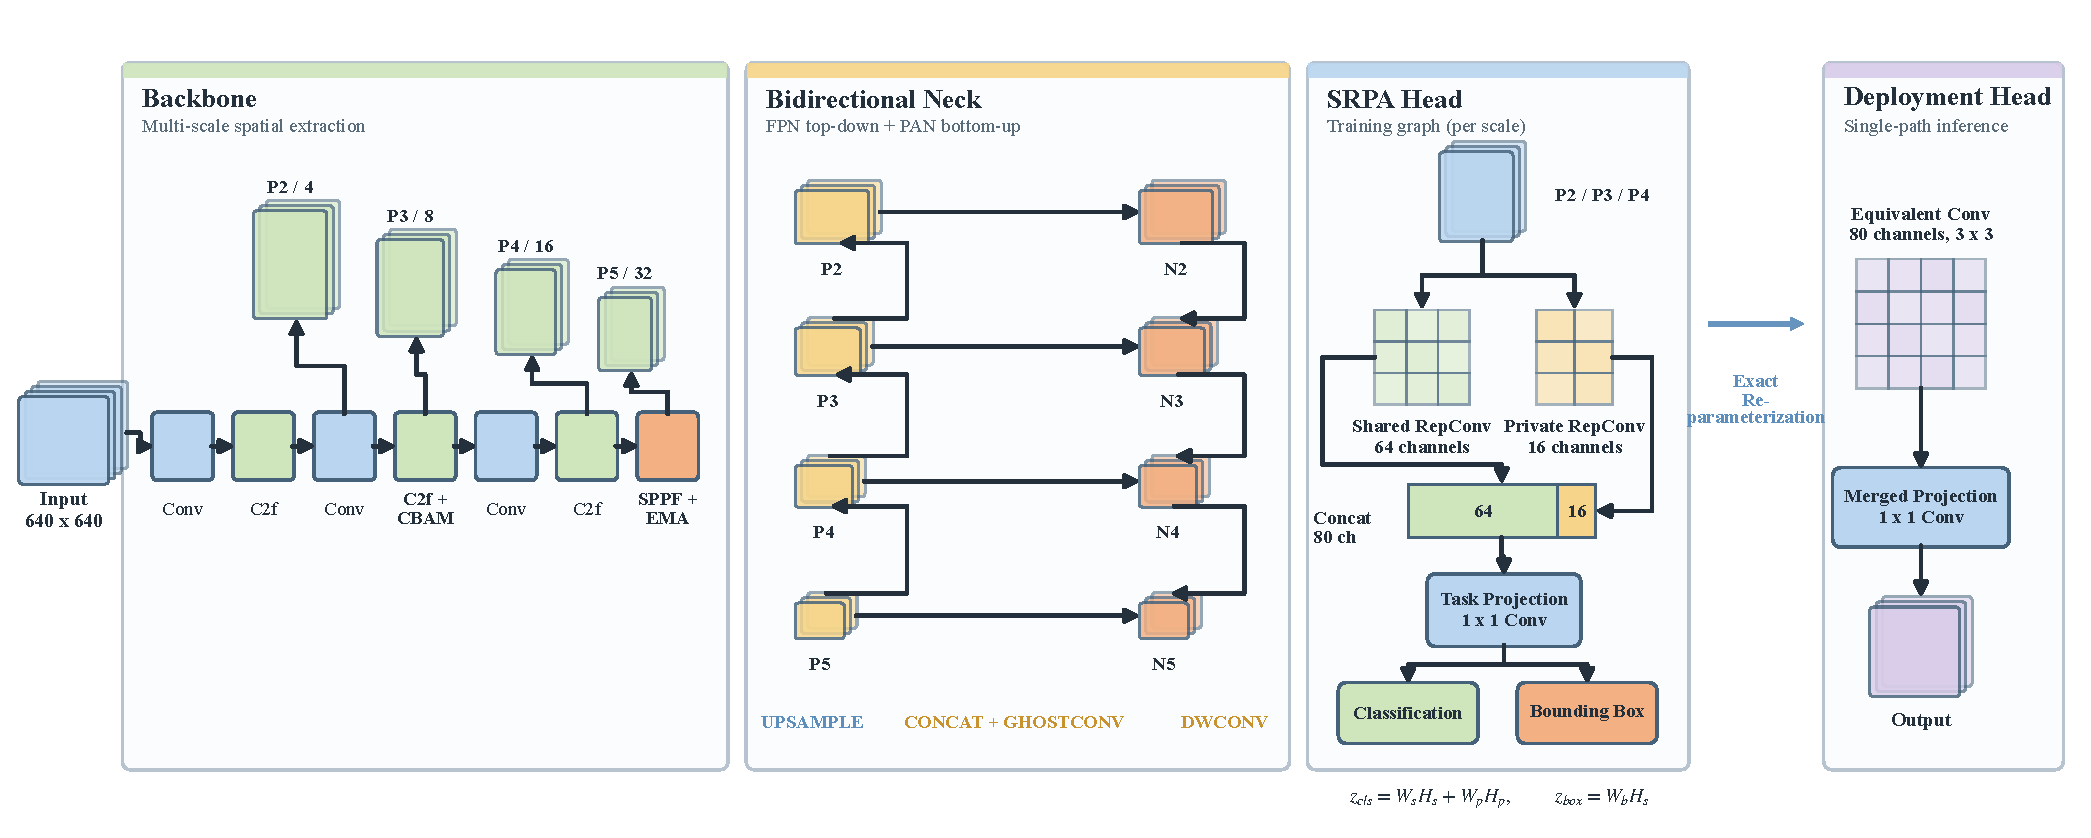
\includegraphics[width=\textwidth]{Fig1.pdf}
\caption{Overall architecture of SRPA-YOLO. The multiscale backbone and bidirectional neck provide P2--P4 features. During training, shared and classification-private representations are optimized separately; exact fusion converts them into a single static deployment path\label{fig:network}}
\end{figure*}

\subsubsection{Multiscale Spatial Feature Extraction}
Let $X_0\in\mathbb{R}^{3\times640\times640}$ be the input image. At backbone stage $l$, the feature map is written as
\begin{equation}
X_l=\mathcal{B}_l(X_{l-1})=\mathcal{A}_l\!\left(\operatorname{BN}(K_l*X_{l-1}+b_l)\right),
\label{eq:backbone}
\end{equation}
where $K_l$ denotes the spatial convolution, $\operatorname{BN}$ denotes batch normalization, and $\mathcal{A}_l$ contains the SiLU activation and local C2f aggregation. The resulting P2, P3, P4, and P5 features have strides $s_l\in\{4,8,16,32\}$. For a target whose transformed maximum side is $d$ pixels, its approximate support on level $l$ is
\begin{equation}
n_l=\frac{d}{s_l}.
\label{eq:targetsupport}
\end{equation}
Retaining P2 therefore gives a $d=8$ pixel UAV approximately two feature cells instead of one cell at stride 8. This higher spatial sampling density reduces the probability that an extremely small target is eliminated before prediction.

\subsubsection{Lightweight Bidirectional Feature Fusion}
The neck combines top-down semantic propagation and bottom-up spatial aggregation. For adjacent pyramid levels, the top-down feature $T_l$ and bottom-up feature $N_l$ are
\begin{equation}
T_l=\psi_l\!\left(\left[X_l,\operatorname{Up}(T_{l+1})\right]\right),\qquad
N_l=\eta_l\!\left(\left[T_l,\operatorname{Down}(N_{l-1})\right]\right),
\label{eq:neck}
\end{equation}
where $[\cdot,\cdot]$ denotes channel concatenation, $\operatorname{Up}$ is nearest-neighbor interpolation, $\operatorname{Down}$ is depthwise strided convolution, and $\psi_l$ and $\eta_l$ are compact C2f/Ghost feature mixers. The top-down path transfers semantic context to high-resolution maps, while the bottom-up path restores edge and displacement cues to deeper maps. This bidirectional exchange is particularly useful when a UAV has weak appearance but remains distinguishable through localized spatial contrast.

\subsubsection{Context-Aware Feature Refinement}
The high-resolution stage applies channel--spatial refinement, whereas the deepest stage aggregates a wider context. For a feature $F$, the refined response can be expressed as
\begin{equation}
\begin{aligned}
\widetilde{F}&=F\odot M_c(F)\odot M_s(F),\\
M_c(F)&=\sigma\!\left(g_c(\operatorname{AvgPool}F,\operatorname{MaxPool}F)\right),\\
M_s(F)&=\sigma\!\left(g_s(\operatorname{Avg}_cF,\operatorname{Max}_cF)\right),
\end{aligned}
\label{eq:refinement}
\end{equation}
where $\odot$ is elementwise multiplication, $\sigma$ is the sigmoid function, and $g_c$ and $g_s$ are lightweight channel and spatial transformations. At P2/P3, the spatial term suppresses cloud edges, foliage, and building textures that resemble tiny UAVs. At the deepest level, pooled contextual responses enlarge the effective receptive field and help distinguish an isolated aerial target from repetitive local clutter. These modules form the retained feature extractor; the contribution of this work concerns the task allocation inside the prediction head.

\subsubsection{P2--P4 Prediction Interface}
The bidirectional neck outputs $N_l$ at $l\in\{2,3,4\}$. A scale-specific projection aligns each feature to the head input dimension,
\begin{equation}
\begin{aligned}
F_l&=P_l*N_l,\qquad F_l\in\mathbb{R}^{C_l\times H_l\times W_l},\\
(H_l,W_l)&\in\{(160,160),(80,80),(40,40)\}.
\end{aligned}
\label{eq:headinput}
\end{equation}
The three levels provide dense coverage for tiny and small UAVs while avoiding a runtime P5 prediction branch. The same SRPA allocation is applied independently at every level, allowing task separation without dynamic routing or scale-dependent control flow.

\subsection{Shared Representation and Private-Rank Allocation}
Conventional shared heads expose classification and localization to the same feature dictionary. SRPA instead retains a shared representation for both tasks and assigns a low-rank classification-private representation, as illustrated in Figure~\ref{fig:allocation}.

\begin{figure*}[!t]
\centering
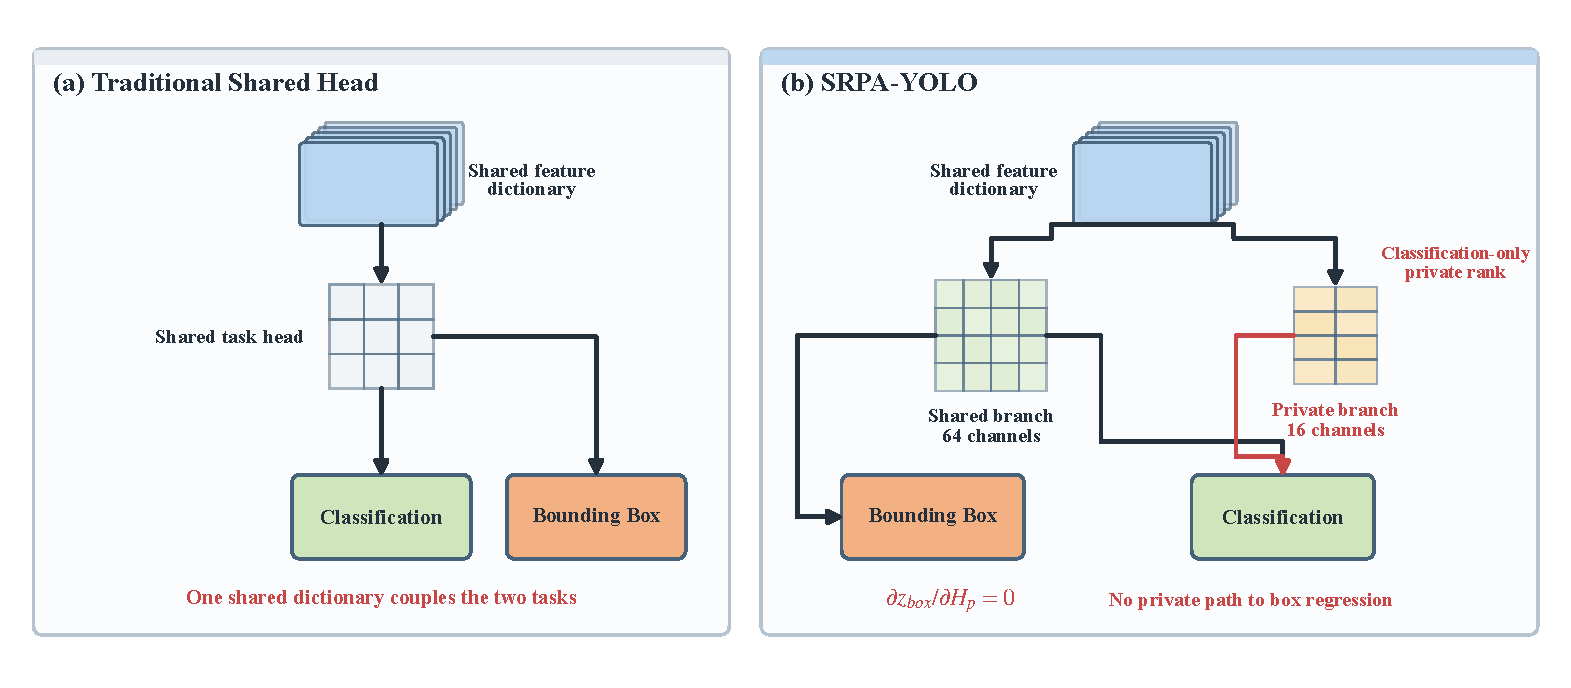
\includegraphics[width=0.86\textwidth]{Fig2.pdf}
\caption{Task-feature allocation in a conventional shared head and the proposed SRPA head. The private representation contributes only to classification, and its Jacobian to the box output is identically zero\label{fig:allocation}}
\end{figure*}

For input feature $F_l$, the shared and classification-private RepConv stems produce
\begin{equation}
H_l^{s}=\phi_s^{(l)}(F_l)\in\mathbb{R}^{64\times H_l\times W_l},\qquad
H_l^{p}=\phi_p^{(l)}(F_l)\in\mathbb{R}^{16\times H_l\times W_l}.
\label{eq:features}
\end{equation}
Let $z_l^{box}$ contain $4K$ DFL logits with $K=16$ bins per coordinate and let $z_l^{cls}$ contain the UAV class logit. SRPA computes
\begin{equation}
z_l^{box}=W_l^{b}H_l^{s}+b_l^{b},
\label{eq:box}
\end{equation}
\begin{equation}
z_l^{cls}=W_l^{s}H_l^{s}+b_l^{s}+W_l^{p}H_l^{p}.
\label{eq:cls}
\end{equation}
Here, the 64 and 16 channels are implementation-level representation dimensions, denoted by $r_s$ and $r_p$ below. They specify the available shared and private channel budgets; they do not assume that a learned convolution attains full algebraic rank. From Equations~\eqref{eq:box} and \eqref{eq:cls},
\begin{equation}
\frac{\partial z_l^{box}}{\partial H_l^{p}}=0,
\label{eq:jacobian}
\end{equation}
which establishes direct computational independence of the box output from the classification-private representation. Upstream task interaction remains mediated by the shared representation learned during Stage I. Flattening spatial dimensions gives $H_l^s\in\mathbb{R}^{r_s\times N_l}$ and $H_l^p\in\mathbb{R}^{r_p\times N_l}$, where $N_l=H_lW_l$. The class-logit row space satisfies
\begin{equation}
\begin{aligned}
z_l^{cls}-b_l^{cls}\mathbf{1}^{\top}
&\in \operatorname{row}(H_l^s)+\operatorname{row}(H_l^p),\\
\dim\!\left(\operatorname{row}(H_l^s)+\operatorname{row}(H_l^p)\right)
&\le r_s+r_p.
\end{aligned}
\label{eq:rowspace}
\end{equation}
Equation~\eqref{eq:rowspace} gives an upper bound on the combined row-space dimension; the attained dimension depends on the learned branch ranks and their subspace overlap. It shows that classification may access up to $r_s+r_p=80$ representation dimensions, whereas localization is computed only from the $r_s=64$ shared dimensions. The private class projection is initialized as $W_l^p=0$, which, provided that the shared detector is unchanged at insertion, yields the function-preserving condition
\begin{equation}
f_{\mathrm{SRPA}}(x;W^p=0)=f_s(x),\qquad \forall x.
\label{eq:identity}
\end{equation}
The expanded detector therefore begins refinement from the trained shared detector with an identical prediction function. During private refinement, the backbone, neck, shared stems, box projections, and shared class projections remain fixed; only $\phi_p$ and $W^p$ are optimized. This constraint leaves the established localization mapping unchanged in Stage II while providing additional class-specific capacity for low-contrast UAVs.

\subsection{Exact Structural Re-Parameterization}
Each RepConv stem contains linear convolution and normalization branches during training. A convolution kernel $K$ followed by batch normalization parameters $(\gamma,\beta,\mu,\sigma^2)$ is converted to
\begin{equation}
\widehat{K}=\frac{\gamma}{\sqrt{\sigma^2+\epsilon}}K,\qquad
\widehat{b}=\beta+\frac{\gamma}{\sqrt{\sigma^2+\epsilon}}(b-\mu).
\label{eq:bnfusion}
\end{equation}
After padding branch kernels to $3\times3$, equivalent branch kernels and biases are summed. Denote the resulting shared and private stems by $(K_s,b_s)$ and $(K_p,b_p)$, where $K_s\in\mathbb{R}^{64\times C\times3\times3}$ and $K_p\in\mathbb{R}^{16\times C\times3\times3}$. Their exact channel-wise fusion is
\begin{equation}
K_d=\begin{bmatrix}K_s\\K_p\end{bmatrix},\qquad
b_d=\begin{bmatrix}b_s\\b_p\end{bmatrix}.
\label{eq:stemfuse}
\end{equation}
For $K=16$ DFL bins and $n_c=1$ class, the corresponding $1\times1$ projections have $W_b\in\mathbb{R}^{4K\times64\times1\times1}$, $W_s\in\mathbb{R}^{n_c\times64\times1\times1}$, and $W_p\in\mathbb{R}^{n_c\times16\times1\times1}$. The deployed projections become
\begin{equation}
W_{box}^{d}=\begin{bmatrix}W_b&0\end{bmatrix},\qquad
W_{cls}^{d}=\begin{bmatrix}W_s&W_p\end{bmatrix}.
\label{eq:projfuse}
\end{equation}
For $H=[H_s;H_p]$, zero-padding the private columns of $W_{box}^{d}$ gives $W_{box}^{d}H=W_bH_s$, while concatenating the class projections gives $W_{cls}^{d}H=W_sH_s+W_pH_p$. The training-time decomposition is therefore converted into one 80-channel $3\times3$ convolution and one merged $1\times1$ projection per scale without changing the computed output apart from floating-point roundoff. Figure~\ref{fig:reparam} summarizes this process.

\begin{figure}[!t]
\centering
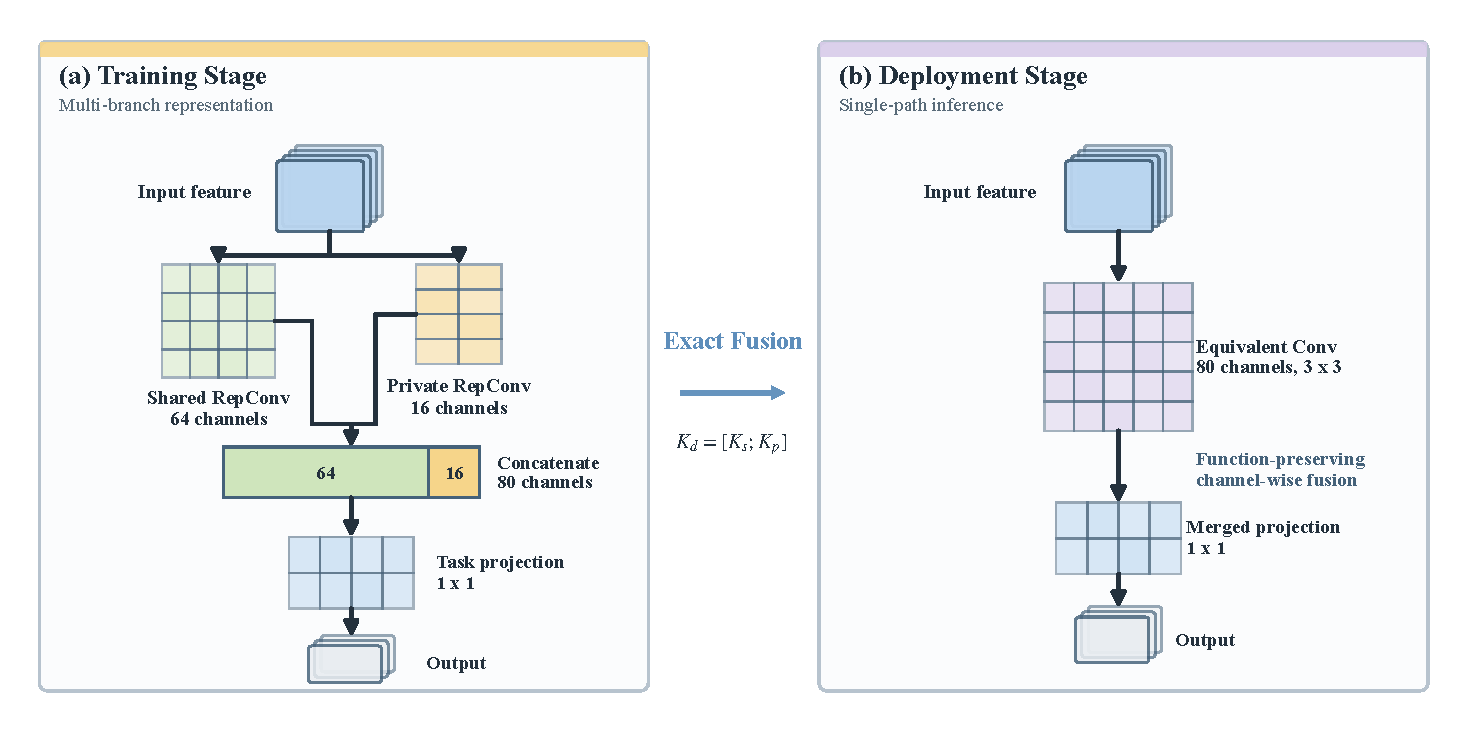
\includegraphics[width=0.92\columnwidth]{Fig3.pdf}
\caption{Structural re-parameterization of the SRPA head. Parallel training representations provide task-specific capacity, while exact kernel and projection fusion produces a single-path deployment graph\label{fig:reparam}}
\end{figure}

Figure~\ref{fig:srpahead} details the single-scale head and its task-specific projections.

\begin{figure}[!t]
\centering
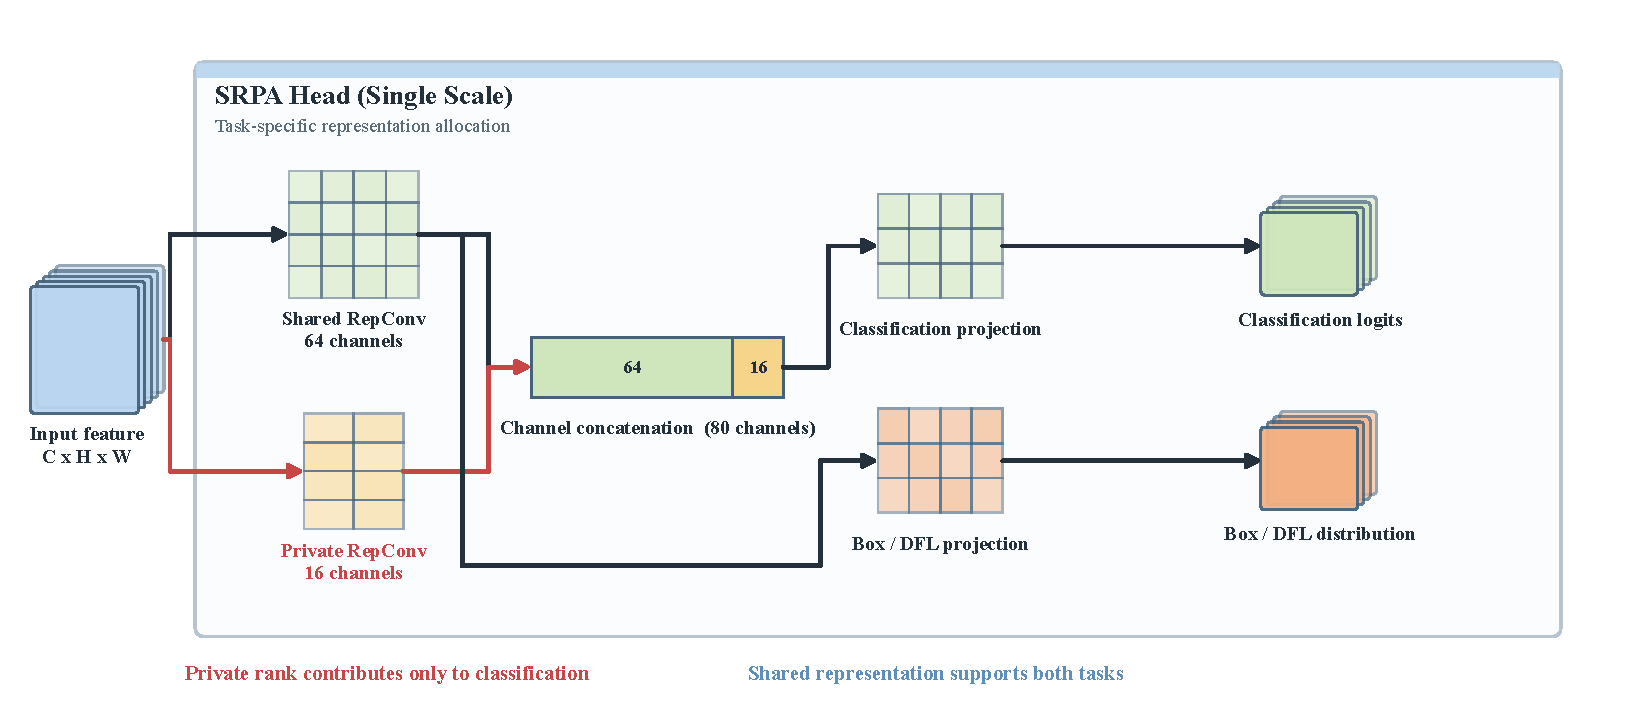
\includegraphics[width=0.92\columnwidth]{Fig4.pdf}
\caption{Internal structure of the SRPA head. Shared features feed both output tasks, while the 16-channel private representation supplies an additive classification residual before deployment fusion\label{fig:srpahead}}
\end{figure}

\subsection{Objective Function and Two-Stage Optimization}
The supervised objective is
\begin{equation}
\begin{aligned}
\mathcal{L}_{sup}={}&\lambda_{box}\mathcal{L}_{CIoU}
+\lambda_{cls}\mathcal{L}_{BCE}
+\lambda_{dfl}\mathcal{L}_{DFL},\\
(\lambda_{box},\lambda_{cls},\lambda_{dfl})={}&(7.5,0.5,1.5),
\end{aligned}
\label{eq:sup}
\end{equation}
where CIoU combines overlap, center-distance, and aspect-ratio penalties \cite{rezatofighi2019giou,zheng2020diou}; BCE supervises class confidence; and DFL models each box coordinate as a discrete distribution.

A frozen RLRD-YOLO teacher regularizes the shared detector. With temperature $T=2$, class-response distillation is
\begin{equation}
\mathcal{L}_{clsKD}=T^2\operatorname{KL}\!\left(\sigma(z_t^{cls}/T)\,\Vert\,\sigma(z_s^{cls}/T)\right).
\label{eq:clskd}
\end{equation}
For positive locations $\Omega_+$, dense localization distillation and confidence-focused localization distillation are
\begin{equation}
\mathcal{L}_{dflKD}=\frac{1}{N_+}\sum_{j\in\Omega_+}\operatorname{KL}\!\left(P_t^{(j)}\Vert P_s^{(j)}\right),
\label{eq:dflkd}
\end{equation}
\begin{equation}
\mathcal{L}_{focus}=\frac{\sum_{j\in\Omega_+}q_j^2\operatorname{KL}(P_t^{(j)}\Vert P_s^{(j)})}{\sum_{j\in\Omega_+}q_j^2+\epsilon},
\label{eq:focus}
\end{equation}
where $q_j$ is teacher confidence. The Stage-I objective is
\begin{equation}
\mathcal{L}=\mathcal{L}_{sup}+0.25\mathcal{L}_{clsKD}+0.50\mathcal{L}_{dflKD}+0.125\mathcal{L}_{focus}.
\label{eq:total}
\end{equation}
Stage II inserts the zero-output classification-private representation and optimizes only $\phi_p$ and $W^p$ from the function-preserving state in Equation~\eqref{eq:identity}. The teacher remains frozen throughout distillation. This schedule first transfers localization knowledge to the compact shared detector and then refines class confidence while the Stage-II box function is fixed.

\subsection{Experimental Environment and Training Settings}
Detailed training parameters are provided in Table~\ref{tab:environment}.

\begin{table}[H]
\caption{Experimental environment and training settings\label{tab:environment}}
\centering\srpatablesetup
\begin{tabular}{@{}p{0.29\columnwidth}p{0.63\columnwidth}@{}}
\toprule
Item & Setting\\
\midrule
Framework & Ultralytics 8.3.239 / PyTorch 2.9.0\\
CUDA & 12.8\\
GPU & NVIDIA GeForce RTX 5060, 8 GB\\
Input size & $640\times640$\\
Batch size & 32\\
Epochs & 200\\
Optimizer & SGD\\
Initial learning rate & 0.01\\
Momentum & 0.937\\
Weight decay & $5\times10^{-4}$\\
Workers & 2\\
Data augmentation & HSV jitter, horizontal flip, translation, scale, and mosaic\\
\bottomrule
\end{tabular}
\end{table}

\subsection{Metrics and Deployment Measurement}
Precision and Recall are computed as
\begin{equation}
P=\frac{TP}{TP+FP},\qquad R=\frac{TP}{TP+FN}.
\label{eq:pr}
\end{equation}
AP@0.50 and AP@0.75 integrate the precision--recall curve at IoU thresholds 0.50 and 0.75, respectively. The primary metric averages AP over ten thresholds,
\begin{equation}
\mathrm{mAP}_{0.50:0.95}=\frac{1}{10}\sum_{k=0}^{9}\mathrm{AP}_{0.50+0.05k}.
\label{eq:map}
\end{equation}
Evaluation uses batch size 32, confidence floor 0.001, NMS IoU 0.7, and at most 300 detections per image. Matched Stage-II experiments use seeds 40, 41, and 42 with the same Stage-I shared basis and independently initialized classification-private parameters to evaluate the stability of private refinement across different initializations.

For shared/private-width analysis, let $m_c$ and $a_c$ be validation \mapall{} and AP@0.75 for configuration $c$. Configurations within 0.003 of the highest validation \mapall{} form
\begin{equation}
\mathcal{C}_{\epsilon}=\left\{c:m_c\ge \max_j m_j-0.003\right\},
\label{eq:selection}
\end{equation}
and the member with the highest AP@0.75 is selected, with AP@0.50 resolving an exact tie. This rule preserves the primary metric while favoring more accurate localization.

Latency is measured at batch 1 and 640 pixels using FP16, fused convolution, forward inference plus NMS, 80 warm-up iterations, and 300 timed iterations. Each candidate and YOLOv8n are loaded in the same process and measured in alternating AB/BA order on the same GPU. Absolute latency and FPS are reported with the corresponding paired YOLOv8n control.

The real-time design is evaluated at the level of the complete detector path rather than by FLOPs alone. The measured frame time includes model forwarding, prediction decoding, and NMS; CUDA synchronization is applied around each timed iteration. Structural fusion is completed before timing, and no training-only classification-private path, dynamic gate, or auxiliary prediction remains in the deployed graph. The resulting latency is therefore the cost paid by the operational detector. Parameter count is reported together with latency because model storage and memory traffic constrain embedded execution even when arithmetic throughput is sufficient.

\section{Experimental Results}

\subsection{Main Accuracy Comparison}
Table~\ref{tab:main} compares SRPA-YOLO with general-purpose compact detectors and UAV-oriented detectors on the deduplicated DUT Anti-UAV test set. SRPA-YOLO achieves 95.850\% Precision, 92.201\% Recall, 95.185\% AP@0.50, 67.071\% \mapall{}, and 77.329\% AP@0.75. YOLOv8n is the direct structural baseline because SRPA-YOLO retains its one-stage training and deployment framework. Relative to YOLOv8n, SRPA-YOLO improves the five metrics by 3.088, 8.242, 5.057, 6.895, and 9.750 percentage points, respectively, while reducing deployed parameters by 0.842 M. Under the common evaluation protocol, the concurrent Precision and Recall gains make an explanation based solely on a shifted confidence operating point less plausible.

\begin{table*}[!t]
\caption{Comparison on 2199 deduplicated DUT Anti-UAV test images. Detection metrics are reported in percent; best values are bold\label{tab:main}}
\centering\srpatablesetup
\begin{tabular}{lrrrrrr}
\toprule
Method & \shortstack{Params\\(M)} & \shortstack{Precision\\(\%)} & \shortstack{Recall\\(\%)} & \shortstack{AP@0.50\\(\%)} & \shortstack{\mapall{}\\(\%)} & \shortstack{AP@0.75\\(\%)}\\
\midrule
YOLO11n & 2.582 & 92.682 & 83.868 & 90.100 & 59.280 & 66.383\\
YOLOv8n & 3.006 & 92.762 & 83.959 & 90.128 & 60.176 & 67.579\\
EDGS-YOLOv8 & 3.091 & 94.266 & 83.244 & 90.428 & 60.347 & 66.415\\
DRBD-YOLOv8 & 3.047 & 92.658 & 83.601 & 90.203 & 60.689 & 67.459\\
YOLOv8n-P2 & 2.921 & \textbf{96.114} & 90.375 & 93.977 & 65.407 & 76.290\\
RLRD-YOLO & 2.926 & 95.781 & 90.107 & 94.467 & 65.436 & 74.757\\
\textbf{SRPA-YOLO} & \textbf{2.164} & 95.850 & \textbf{92.201} & \textbf{95.185} & \textbf{67.071} & \textbf{77.329}\\
\addlinespace
$\Delta$ SRPA vs. YOLOv8n & $-0.842$ & $+3.088$ & $+8.242$ & $+5.057$ & $+6.895$ & $+9.750$\\
\bottomrule
\end{tabular}
\end{table*}


Figure~\ref{fig:comparison} summarizes the accuracy and compactness comparison across the evaluated detectors.

\begin{figure*}[!t]
\centering
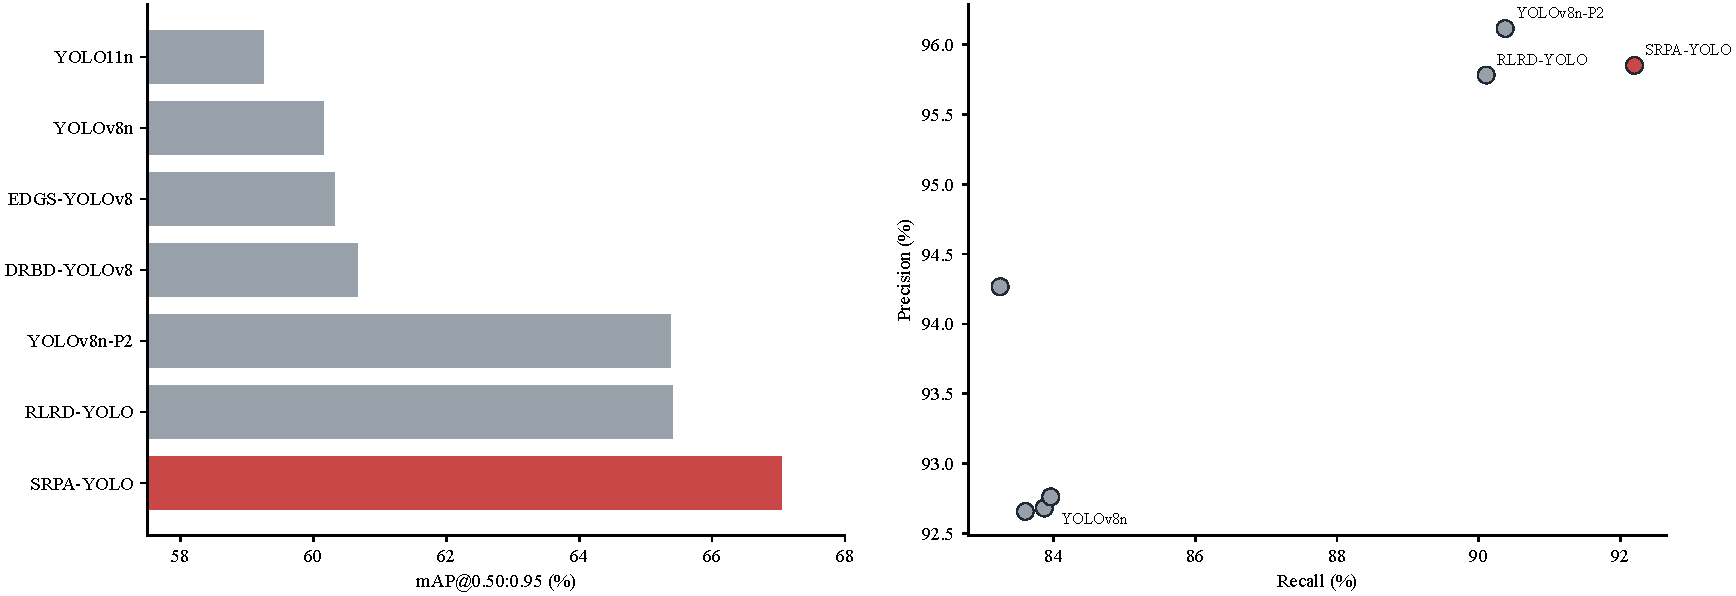
\includegraphics[width=0.86\textwidth]{Fig5.pdf}
\caption{Accuracy and compactness comparison on the deduplicated DUT Anti-UAV test set. All detection metrics are reported in percent.\label{fig:comparison}}
\end{figure*}

YOLOv8n-P2 controls for the effect of adding a high-resolution prediction level. Although its Precision is 0.264 percentage points higher, SRPA-YOLO improves Recall, AP@0.50, \mapall{}, and AP@0.75 by 1.826, 1.208, 1.664, and 1.039 percentage points, respectively. This comparison shows that task-feature allocation inside the detection head contributes additional gains beyond high-resolution scale extension.

Figure~\ref{fig:complexity} relates deployed parameters to the primary accuracy metric. SRPA-YOLO occupies the upper-left region, combining the highest measured \mapall{} with the smallest parameter count among the compared detectors. This operating point is consistent with the design objective of assigning a compact shared dictionary and limiting additional capacity to the classification task.

\begin{figure}[!t]
\centering
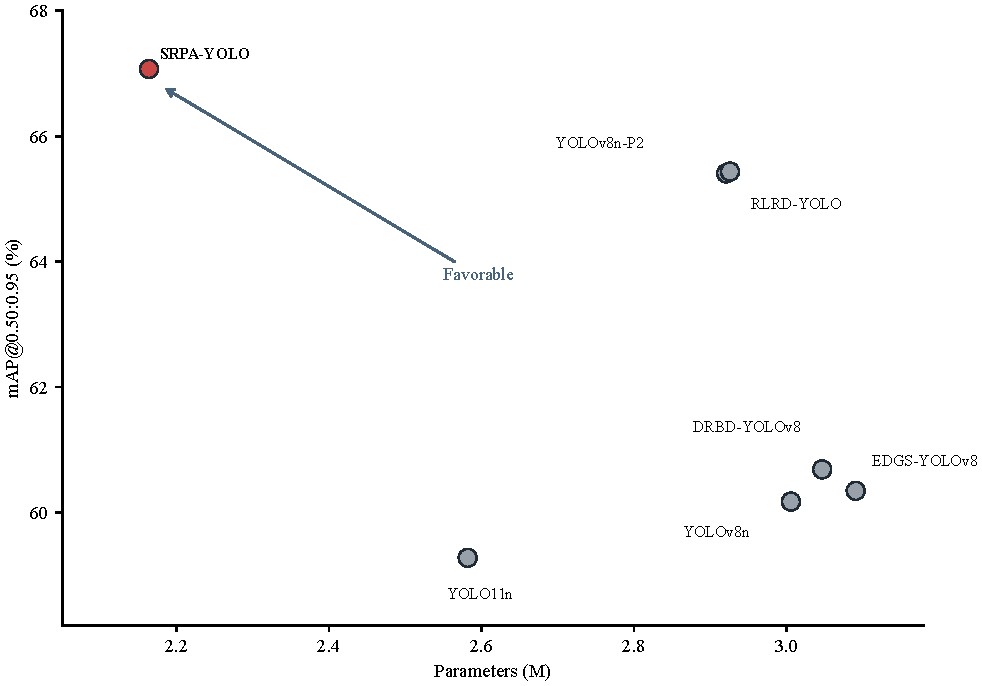
\includegraphics[width=0.90\columnwidth]{Fig6.pdf}
\caption{Model-complexity trade-off. The horizontal axis is deployed parameter count and the vertical axis is \mapall{}.\label{fig:complexity}}
\end{figure}


\subsection{Shared/Private-Rank and Mechanism Ablations}
Table~\ref{tab:rank} isolates the effect of shared and private ranks on the validation set. Increasing the shared rank from 48 to 64 or 80 does not lead to a monotonic increase in \mapall{}, indicating that uniform width expansion is not sufficient to determine the optimum. The 48+16 allocation reaches the highest validation \mapall{} (60.874\%), whereas 64+16 produces the highest AP@0.75 (69.986\%), AP@0.50 (91.850\%), and Precision (96.615\%). According to Equation~\eqref{eq:selection}, both allocations lie within 0.3 percentage points of the highest \mapall{}, and 64+16 is selected because it provides the strongest high-IoU localization.

\begin{table*}[!t]
\caption{Validation-selected shared/private rank ablation. Detection metrics are percentages; $r_s+r_p$ denotes shared rank plus classification-private rank\label{tab:rank}}
\centering\srpatablesetup
\begin{tabular}{rrrrrrr}
\toprule
$r_s$ & $r_p$ & \shortstack{Params\\(M)} & \shortstack{Precision\\(\%)} & \shortstack{Recall\\(\%)} & \shortstack{AP@0.50\\(\%)} & \shortstack{\mapall{} /\\AP@0.75 (\%)}\\
\midrule
48 & 0  & 2.093 & 96.089 & 87.182 & 91.667 & 60.508 / 69.337\\
64 & 0  & 2.128 & 96.378 & 86.570 & 91.703 & 60.454 / 69.754\\
80 & 0  & 2.164 & 96.073 & \textbf{87.743} & 91.569 & 60.513 / 69.262\\
48 & 16 & 2.128 & 96.135 & 87.310 & 91.798 & \textbf{60.874} / 69.618\\
\textbf{64} & \textbf{16} & \textbf{2.164} & \textbf{96.615} & 86.570 & \textbf{91.850} & 60.646 / \textbf{69.986}\\
\bottomrule
\end{tabular}
\end{table*}


Table~\ref{tab:mechanism} traces cumulative changes from a nonlinear head to the final SRPA configuration. Adding dense DFL distillation is associated with recovery from the accuracy loss of head compression, and the subsequent confidence-focused term adds 0.384 \mapall{} points. Under the cumulative protocol, transferred initialization coincides with increases of 2.660 Recall points and 0.678 \mapall{} points; increasing the shared representation to 64 channels is followed by gains of 0.531 \mapall{} points and 1.674 AP@0.75 points. The final 16-channel classification-private representation reaches 67.071\% \mapall{} and 77.329\% AP@0.75. Each row retains the preceding components and therefore reports the performance of the corresponding cumulative configuration. The shared-80 control reaches a similar \mapall{} of 67.121\%, whereas the 64+16 allocation additionally enforces the zero box Jacobian in Equation~\eqref{eq:jacobian} and is selected by the predefined validation localization criterion. Together with the rank ablation, the results support task-constrained capacity allocation instead of unrestricted head widening.

\begin{table*}[!t]
\caption{Mechanism ablation on the deduplicated DUT Anti-UAV test set. Detection metrics are percentages\label{tab:mechanism}}
\centering\srpatablesetup
\begin{tabular}{p{0.27\textwidth}rrrrrr}
\toprule
Configuration & \shortstack{Params\\(M)} & \shortstack{Precision\\(\%)} & \shortstack{Recall\\(\%)} & \shortstack{AP@0.50\\(\%)} & \shortstack{\mapall{}\\(\%)} & \shortstack{AP@0.75\\(\%)}\\
\midrule
Full nonlinear head & 2.603 & 95.922 & 90.954 & 94.736 & 66.046 & 75.503\\
Shared-48 + dense DFL KD & 2.093 & 96.152 & 90.954 & 94.836 & 65.363 & 74.929\\
$+$ focused localization KD & 2.093 & 97.084 & 90.285 & 95.018 & 65.747 & 75.573\\
$+$ transferred initialization & 2.093 & 96.484 & 92.945 & \textbf{95.493} & 66.425 & 75.472\\
$+$ shared rank 64 & 2.128 & 96.122 & 92.157 & 95.366 & 66.956 & 77.146\\
$+$ private rank 16 & 2.164 & 95.850 & 92.201 & 95.185 & \textbf{67.071} & \textbf{77.329}\\
\bottomrule
\end{tabular}
\end{table*}



\subsection{Localization and Scale Characteristics}
Figure~\ref{fig:scaleiou} compares SRPA-YOLO directly with YOLOv8n over IoU thresholds from 0.50 to 0.95. SRPA-YOLO has higher AP at every threshold. The margin is 5.057 percentage points at IoU 0.50, increases to 9.750 points at IoU 0.75, and remains 8.803 points at IoU 0.85. The persistence of the margin under stricter overlap criteria indicates that the measured improvement includes a localization component and is not confined to class confidence at IoU 0.50.

\begin{figure*}[!t]
\centering
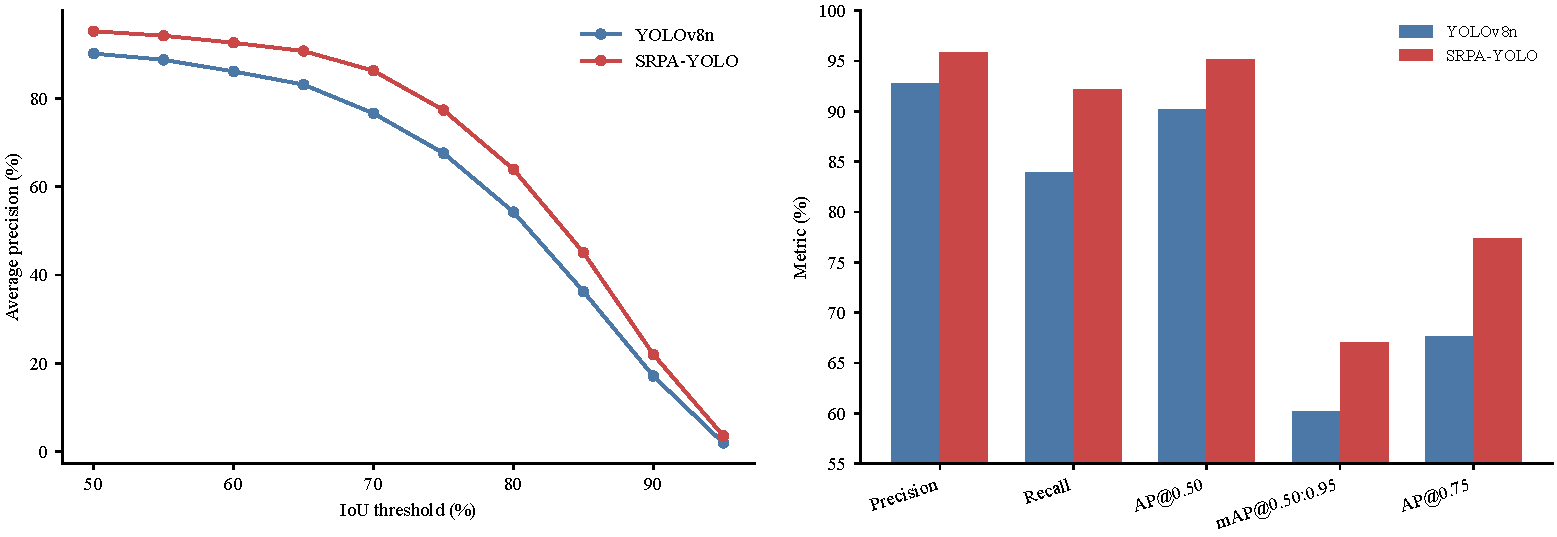
\includegraphics[width=0.84\textwidth]{Fig7.pdf}
\caption{Localization comparison between SRPA-YOLO and YOLOv8n. Left: AP at individual IoU thresholds; right: aggregate detection metrics.\label{fig:scaleiou}}
\end{figure*}

The largest aggregate improvement over YOLOv8n is observed in Recall (+8.242 points), accompanied by gains in both AP@0.50 and AP@0.75. In long-range UAV monitoring, improved Recall directly reduces missed targets, while the concurrent Precision increase limits additional false alarms. The P2 prediction level provides spatial support for tiny UAVs, while the SRPA head keeps classification-private refinement outside the box-regression input. This structural interpretation is consistent with the observed gains at both low and high IoU thresholds.


\subsection{Qualitative Detection Analysis}
Figure~\ref{fig:detectioncomparison} compares YOLOv8n and SRPA-YOLO on the same tiny-UAV instances at a confidence threshold of 0.25. A detection is regarded as correct when its IoU with the ground-truth box is at least 0.50. In all three selected examples, YOLOv8n produces no matched prediction, whereas SRPA-YOLO recovers the target. These representative cases visually corroborate the quantitative improvements reported on the test set. The enlarged regions show the spatial alignment of the recovered predictions for targets represented by only a few pixels.

\begin{figure*}[!t]
\centering
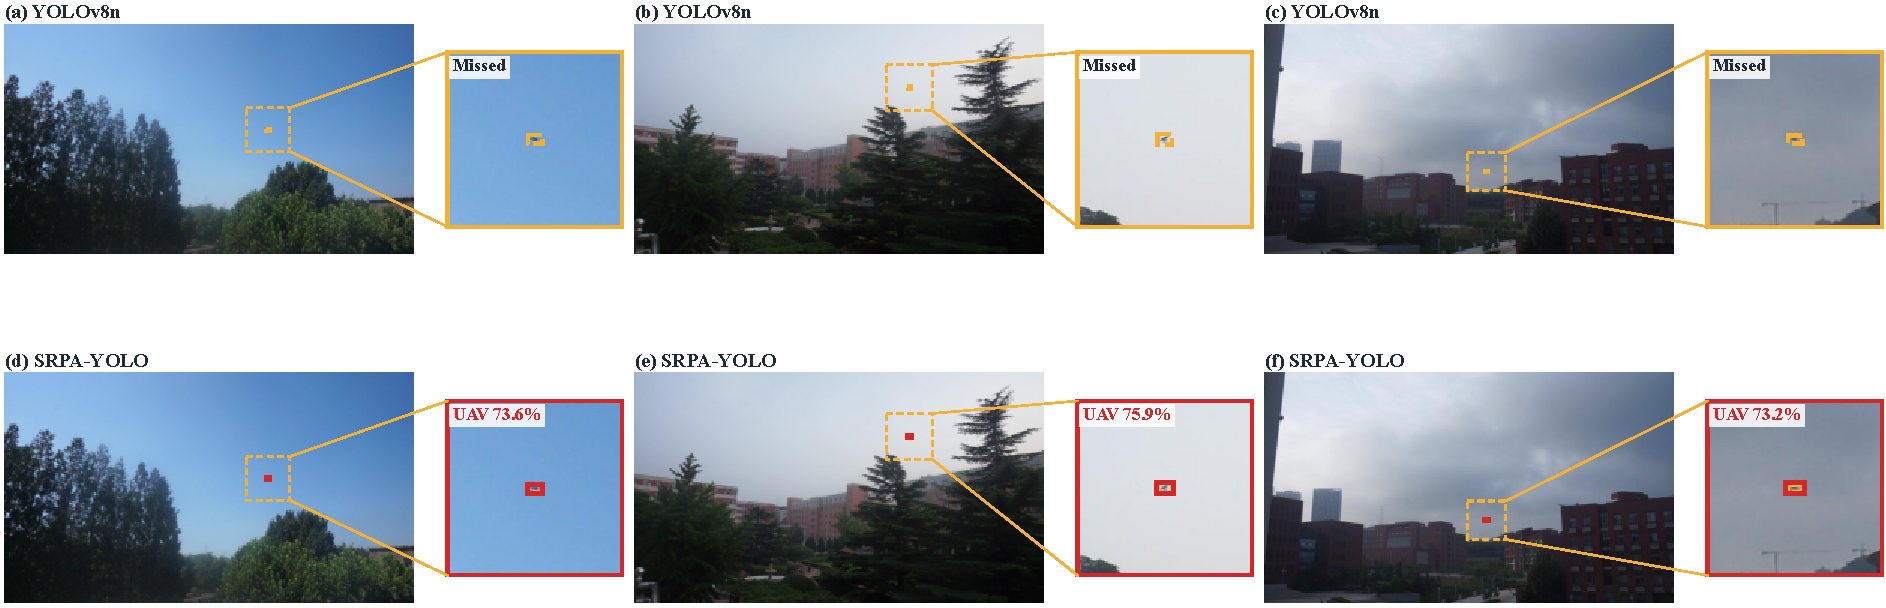
\includegraphics[width=0.84\textwidth]{Fig8.pdf}
\caption{Matched-image detection comparison on the deduplicated DUT Anti-UAV test set. Yellow dashed boxes denote ground truth, red solid boxes denote SRPA-YOLO predictions, and ``Missed'' indicates that YOLOv8n has no prediction satisfying confidence $\geq0.25$ and IoU $\geq0.50$.\label{fig:detectioncomparison}}
\end{figure*}

Figure~\ref{fig:tinydetections} further presents successful SRPA-YOLO detections under sky, building, vegetation, and low-contrast backgrounds. The selected targets have projected longest-edge lengths of 5.7--6.3 pixels after 640-pixel letterboxing. Despite the limited target support and substantial surrounding background, the final validation-selected checkpoint produces localized responses in each selected scene. These cases illustrate the model's small-target detection behavior and are consistent with the preceding test-set metrics.

\begin{figure*}[!t]
\centering
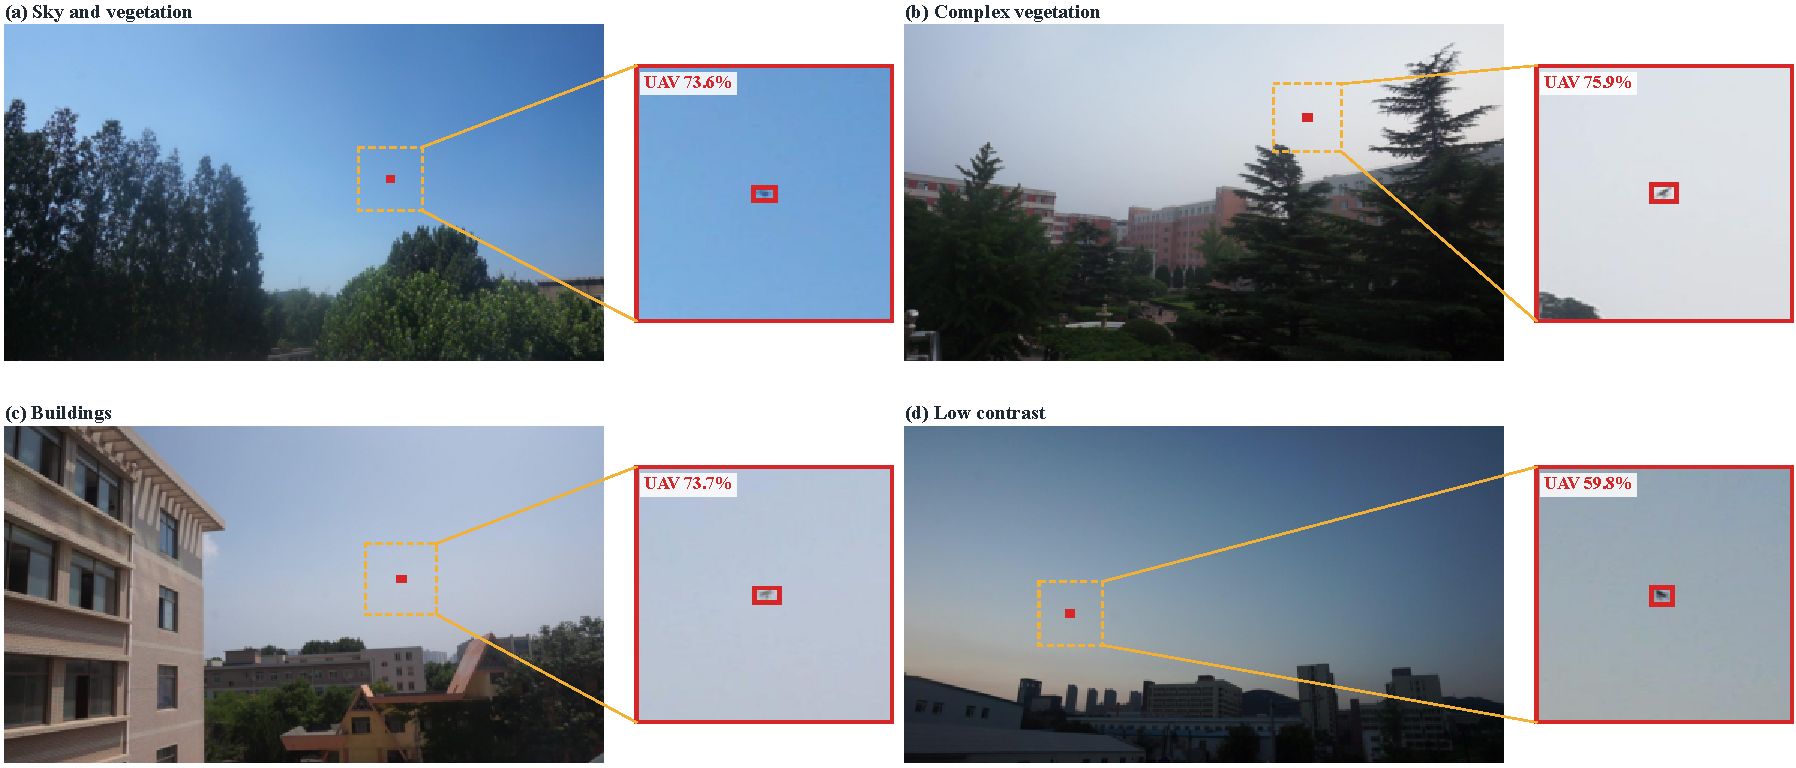
\includegraphics[width=0.74\textwidth]{Fig9.pdf}
\caption{Successful SRPA-YOLO detections of tiny UAVs. Each right-hand view enlarges the target region from the corresponding full image; red boxes and labels are predictions from the final validation-selected checkpoint.\label{fig:tinydetections}}
\end{figure*}


\subsection{Matched-Seed Stability}
Table~\ref{tab:seeds} summarizes the results for Stage-II seeds 40, 41, and 42. All experiments use the same Stage-I shared basis and independently initialize the classification-private parameters. SRPA-YOLO yields standard deviations of 0.112, 0.022, and 0.082 percentage points for Recall, AP@0.50, and \mapall{}, respectively, indicating low variation across these private-parameter initializations. Relative to RLRD-YOLO, the mean paired differences in Recall, \mapall{}, and AP@0.75 are +2.709, +1.881, and +2.150 percentage points, respectively. Under the matched protocol, the observed improvement is consistent across the three Stage-II seeds.

\begin{table}[H]
\caption{Matched Stage-II seeds on the deduplicated DUT Anti-UAV test set (percent, mean $\pm$ sample standard deviation, $n=3$). All runs use the same Stage-I shared basis and independently initialize only the private parameters\label{tab:seeds}}
\centering\srpatablesetup
\begin{tabular}{@{}lrrr@{}}
\toprule
Metric (\%) & RLRD-YOLO & SRPA-YOLO & Paired diff.\\
\midrule
Precision & $95.964\pm0.766$ & $\mathbf{96.167\pm0.031}$ & $+0.204\pm0.736$\\
Recall & $89.463\pm0.785$ & $\mathbf{92.172\pm0.112}$ & $+2.709\pm0.773$\\
AP@0.50 & $94.661\pm0.106$ & $\mathbf{95.304\pm0.022}$ & $+0.644\pm0.109$\\
\mapall{} & $65.199\pm0.639$ & $\mathbf{67.080\pm0.082}$ & $+1.881\pm0.721$\\
AP@0.75 & $75.196\pm0.564$ & $\mathbf{77.345\pm0.233}$ & $+2.150\pm0.332$\\
\bottomrule
\end{tabular}
\end{table}
\vspace{-4pt}



\subsection{Latency and Deployment Complexity}
The training graph contains approximately 2.18 M parameters and requires 8.5 GFLOPs at 640 pixels. Structural fusion removes training-only state and produces a 2.164 M-parameter checkpoint. Table~\ref{tab:latency} reports same-process paired measurements, in which each detector is evaluated together with a paired YOLOv8n control; Table~\ref{tab:cleanlat} gives the separate low-load final-acceptance measurements.

\begin{table}[!t]
\caption{Same-process paired latency. Each row reports a candidate and its paired YOLOv8n control; batch 1, 640 pixels, FP16, fused forward+NMS, 80 warm-ups, and 300 iterations\label{tab:latency}}
\centering\srpatablesetup
\begin{tabular}{@{}lrrrr@{}}
\toprule
Method & Round & ms & FPS & Control ms\\
\midrule
YOLO11n & 1 & 21.6357 & 46.22 & 16.8632\\
 & 2 & 19.1505 & 52.22 & 15.0139\\
YOLOv8n-P2 & 1 & 19.1953 & 52.10 & 15.9227\\
 & 2 & 16.9629 & 58.95 & 14.1962\\
EDGS* & 1 & 19.5146 & 51.24 & 14.6088\\
 & 2 & 22.0043 & 45.45 & 16.3604\\
DRBD* & 1 & 29.0158 & 34.46 & 14.5733\\
 & 2 & 31.7115 & 31.53 & 16.8584\\
RLRD-YOLO & 1 & 22.5644 & 44.32 & 16.0771\\
 & 2 & 22.7773 & 43.90 & 16.2647\\
\textbf{SRPA-YOLO} & \textbf{1} & \textbf{16.2469} & \textbf{61.55} & 16.4922\\
 & \textbf{2} & \textbf{15.0936} & \textbf{66.25} & 15.5909\\
\bottomrule
\end{tabular}
\end{table}

\begin{table}[!t]
\caption{Separate low-load final-acceptance measurements for SRPA-YOLO and its paired YOLOv8n control under the same batch-1, 640-pixel, FP16, fused forward+NMS protocol\label{tab:cleanlat}}
\centering\srpatablesetup
\begin{tabular}{@{}lrrrr@{}}
\toprule
Round & \shortstack{SRPA\\ms} & \shortstack{SRPA\\FPS} & \shortstack{YOLOv8n\\ms} & \shortstack{YOLOv8n\\FPS}\\
\midrule
1 & \textbf{9.7435} & \textbf{102.63} & 9.8859 & 101.15\\
2 & \textbf{9.8574} & \textbf{101.45} & 9.9893 & 100.11\\
\bottomrule
\end{tabular}
\end{table}


In the separate low-load acceptance measurements, SRPA-YOLO requires 9.7435 and 9.8574 ms (102.63 and 101.45 FPS), whereas the paired YOLOv8n control requires 9.8859 and 9.9893 ms (101.15 and 100.11 FPS). The two-round means are 9.8005 ms and 9.9376 ms, respectively. Under the reported protocol, SRPA-YOLO achieves comparable frame time while reducing the deployed parameter count by 28.0\%.

Figure~\ref{fig:speedtradeoff} combines the reported two-round mean latency with the primary accuracy metric. Among the measured models and under this hardware protocol, SRPA-YOLO occupies the favorable accuracy--speed boundary: models with comparable accuracy have higher measured latency, whereas faster models do not reach the same \mapall{}.

\begin{figure}[!t]
\centering
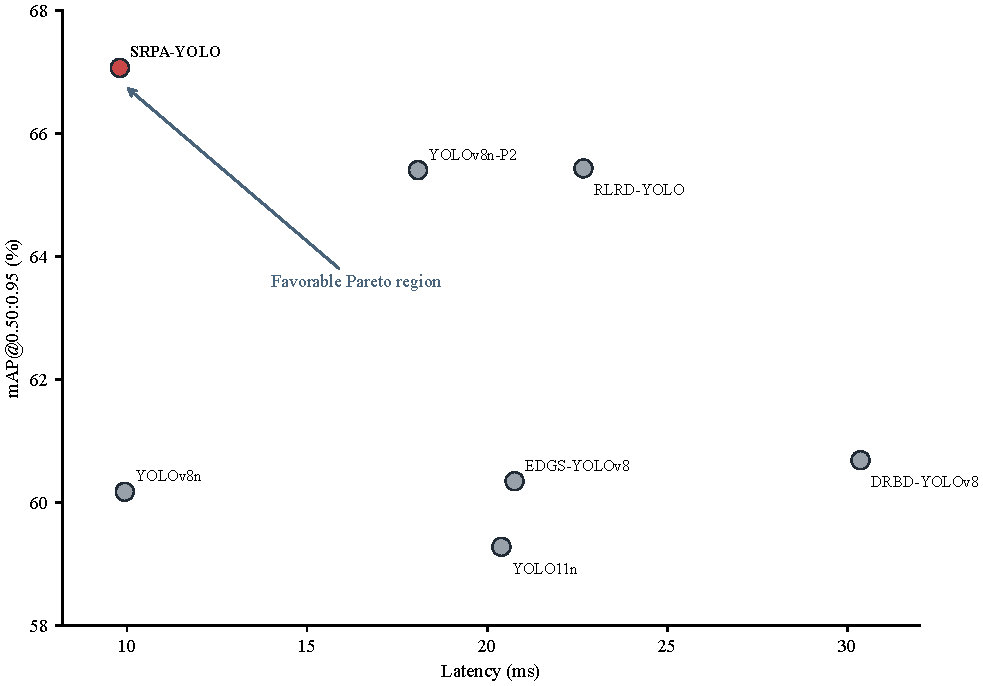
\includegraphics[width=0.72\columnwidth]{Fig10.pdf}
\caption{Accuracy--speed trade-off based on the reported two-round mean latency and \mapall{}.\label{fig:speedtradeoff}}
\end{figure}

\FloatBarrier

\section{Conclusions}

This paper presented SRPA-YOLO, a compact detector that formulates prediction-head capacity as task-specific representation allocation. A 64-channel shared representation supports classification and DFL localization, whereas a zero-output-initialized 16-channel classification-private representation contributes only an additive class residual. This construction increases the feature capacity available to classification while making the box output directly independent of the private representation. Exact structural re-parameterization converts the training-time decomposition into one 80-channel convolution and one merged output projection per scale, yielding a static single-path deployment graph.

On the deduplicated DUT Anti-UAV test set, the selected checkpoint achieves 95.850\% Precision, 92.201\% Recall, 95.185\% AP@0.50, 67.071\% \mapall{}, and 77.329\% AP@0.75 with 2.164 M deployed parameters. Compared with YOLOv8n, the corresponding improvements are 3.088, 8.242, 5.057, 6.895, and 9.750 percentage points, together with 28.0\% fewer parameters. The additional gains in Recall, AP@0.50, \mapall{}, and AP@0.75 over YOLOv8n-P2 show that head-level task allocation complements high-resolution prediction. The gains across the evaluated IoU thresholds and the low variation in the matched-seed experiments are consistent with stable localization and classification refinement under the reported protocol.

Two paired deployment measurements yield 9.7435 and 9.8574 ms for SRPA-YOLO and 9.8859 and 9.9893 ms for the paired YOLOv8n control under the specified RTX 5060, FP16, batch-1, forward-plus-NMS protocol. Together with the 28.0\% parameter reduction, these measurements indicate a favorable accuracy--compactness operating point on the evaluated GPU software stack. Future work should examine multi-class aerial scenes, embedded ONNX/TensorRT deployment, and scale-conditioned private capacity under additional target-size and imaging conditions.

\section*{Statements and Declarations}

\noindent\textbf{Funding.} The authors declare that no funds, grants, or other support were received during the preparation of this manuscript.

\noindent\textbf{Competing interests.} The authors have no relevant financial or non-financial interests to disclose.

\noindent\textbf{Author contributions.} Xianpu Wang: conceptualization, methodology, software, validation, formal analysis, investigation, data curation, visualization, and writing---original draft. Haijie Zhi: validation, formal analysis, and writing---review and editing. Qing Fei: conceptualization, supervision, resources, project administration, and writing---review and editing. All authors read and approved the final manuscript.

\noindent\textbf{Data and code availability.} The DUT Anti-UAV dataset is available from its public project repository subject to the provider's terms. The reproducibility package contains the deduplication manifest, source code, model configurations, result manifest, paired-latency records, and editable plotting scripts. These materials and the trained weights are available from the corresponding author and will be deposited in a versioned public repository. One cross-split duplicate is excluded by a fixed manifest and documented by its SHA-256 hash; no source image is deleted.

\begin{acknowledgements}
The authors thank the maintainers of the DUT Anti-UAV benchmark and the Ultralytics open-source framework.
\end{acknowledgements}


\bibliographystyle{spmpsci}
\bibliography{../bibliography/references}

\end{document}
